% -*- coding: utf-8 -*-
\newpage
\section{Testing and Performance}

To validate the new implementation, we performed extensive tests across a wide
range of systems, aiming both to push the code to its limits and to ensure its
robustness. These tests also allowed us to compare the performance of the
current version with other programs and with the previous
implementation.

\subsection{Exotic and Complex Topologies}

To assess the limits of the code, we selected systems that had previously been
reported as problematic in earlier versions, as well as examples from the
literature known to present topologically challenging cases.

\subsubsection{Grid Refinement}

\begin{wrapfigure}[9]{r}{0.5\textwidth}
  \centering
  \includegraphics[width=0.5\textwidth]{img/ferrocene_cp_cartoon.png}
  \caption{Ferrocene with its \glspl{RCP}. The \glspl{RCP} highlighted in yellow were not
           detected in the previous version of the code. Due to molecular
           symmetry, any of the \glspl{RCP} could be among those missing.}
  \label{img_ferrocene}
\end{wrapfigure}

In earlier versions, the default grid settings failed to satisfy the
Poincaré-Hopf relation for systems such as H$_2$. The single
\gls{BCP} in this molecule requires a finer grid for reliable detection. This
issue was not restricted to small systems; more complex molecules, such as
ferrocene, ($\eta^5$-C$_5$H$_5$)$_2$Fe, also exhibited undetected
\glspl{CP} when using default grid parameters.

\subsubsection{Gradient Path Algorithm}

To further test the limits of the code, we examined two systems in which the
electron density exhibits a relatively flat profile, making the algorithm used
to follow the gradient path crucial for correctly determining how the atoms are
bonded: $i$) the transition state of the Diels–Alder reaction of
cyclopentadiene, and  $ii$) the Be$_3^{-2}$ system. It is worth noting that
\gls{QTAIM} analysis is not restricted to neutral or minimum-energy states.

In case $i$), illustrated in Figure~\ref{diels_alder}, the transition state
features a complex topology, a Diels-Alder transition state between two
molecules of cyclopentadiene, dicyclopentadiene as product. Here, fine grid
refinement was not required to detect all \glspl{CP} with BLYP/DZ,
however, it was required for M06-2X/TZP. The use of fourth-order
Runge-Kutta was essential for accurately tracing the gradient paths within the
rings. While the two C-rings are clearly resolved as well as the cage, several
additional \glspl{RCP} appear in the topology, which can be attributed to the
bond-forming and bond-breaking processes occurring at the transition state.

\vspace*{0.7cm}%
\begin{figure}[h]
  % \centering
  \begin{subfigure}[t]{0.63\textwidth}
    \centering
    \includegraphics[width=0.63\textwidth]{img/dielsAlder.png}
    \caption{The non-trivial \glspl{RCP} (green
      spheres) are shown with their constituent atoms, with the associated paths
      highlighted in yellow, magenta, and cyan for clarity. The \gls{CCP} (blue
      sphere) connects all carbon atoms. For simplicity, the two \glspl{RCP}
      associated with the cyclopentadiene rings (considered as trivial) are omitted.
      Cartesian coordinates are provided in Appendix~\ref{xyzfiles}.}
    \label{diels_alder}
  \end{subfigure}
  \hfill%
  \begin{subfigure}[t]{0.34\textwidth}
    \centering
    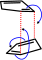
\includegraphics[width=0.75\textwidth]{img/da_flechas.pdf}
    \caption{Mechanism of reaction of the Diels-Alder transition state, in
      standard organic chemistry notation.}
    \label{da_flechas}
  \end{subfigure}
  \caption{Diels-Alder transition state. The creation of bonds noted by dashed lines
    in Figure~\ref{da_flechas} is reflected in the ring highlighted in yellow
    in Figure~\ref{diels_alder}.}
\end{figure}

\newpage
In case $ii$), we investigated the Be$_3^{-2}$ system as a function of basis
set, functional, and interatomic distance, as this system has previously been
reported to exhibit complex topology~\cite{Goswami2015}. The model consisted of
an equilateral triangle of Be atoms, with the side length varied
systematically. This analysis revealed that the number of \glspl{CP} changes
in function with both geometry and level of theory, including NNA. In the
previous code version, some of the systems do not satisfy the Poincaré-Hopf
relation, and in some of them the gradient path goes two times to the same atom
or to no any.

In contrast, the improved algorithm in the current version consistently
identifies all \glspl{CP} and follows the gradient paths correctly. It is
important to note that sometimes the refinement of the grid was required until
the grid spacing was 0.013~bohr, which is a significant fine grid, we proposed
to use 0.1~bohr for the new default grid spacing (used to be 0.5~bohr). This
change will contemplate most of the systems.

To illustrate the performance, we display the case of the Be$_3^{-2}$ system
with $1.960$~\AA\ interatomic distance between the Be atoms, using the B3LYP
functional and DZP basis set (Figure~\ref{beTriang}). For the previous version,
the code finds the NNA, six \glspl{BCP}, and only one \glspl{RCP}, no any of
the gradient paths goes to anywhere. The current version finds the same NNA,
six \glspl{BCP}, but also the three \glspl{RCP}, as well following the paths
from the \glspl{BCP} to the atoms, properly.

\begin{figure}[hb!]
  % \centering
  \begin{subfigure}[t]{0.45\textwidth}
    \centering
    \includegraphics[width=\textwidth]{img/nna_no.png}
    \caption{Every connection from the Be atoms to the NNA have two \glspl{BCP}, but
      only one has the \glspl{RCP} that should appear between the two \gls{BCP}. The gradient
      paths simply do not appear, since they do not go to anywhere.}
    \label{OldVersion}
  \end{subfigure}
  \hfill%
  \begin{subfigure}[t]{0.45\textwidth}
    \centering
    \includegraphics[width=\textwidth]{img/nna_yes_cropped.png}
    \caption{All \glspl{BCP} as well as the \glspl{RCP} are found, and all the gradient
      paths go from the Be atoms to the NNA.}
    \label{NewVersion}
  \end{subfigure}
  \caption{Comparison of the Be$_3^{-2}$ system with 1.960~\AA\ interatomic distance
    between the Be atoms, using B3LYP/DZP. Images generated directly from the \ams \gls{GUI}.
    The \glspl{BCP} are shown in red, the \glspl{RCP} in green.}
  \label{beTriang}
\end{figure}

% \newpage
\subsection{Numerical Comparison}

Following the refactoring of the code, it was essential to verify that the new
version reproduces the same physical properties as the previous one. While
minor numerical differences are expected as a result of the refactoring, the
underlying physical trends must remain unchanged.

For atomic properties already implemented in earlier versions, where the only
modifications arose from code refactoring, we used the built-in tools of the
\ams development environment to compare the results of the new implementation
with those of the most recent stable and well-documented version. The
differences in numerical values were on the order of $10^{-15}$, well below the
threshold of numerical noise, and were ignored by the comparison tools.

\lstset{style=terminal, numbers=none, escapeinside={(*@}{@*)}}
\begin{macterminal}[victoria@rameau - bash]
$ # Compare the results of the new code with the previous version
$ cd $AMSHOME
$ for keyword in IQA Bader QTAIM; do
~  ./Utils/run_where $keyword
~ done
$ # Summary files
$ ls diffs.*
\end{macterminal}
\lstset{style=mystyle}

In contrast to the properties affected only by refactoring, the atomic dipole
moments have no direct counterpart in previous versions of the code, and must
therefore be validated against external implementations. For this purpose, we
computed 34~k molecular systems ($\sim$468~k atoms) using \adf and compared the
results with those obtained from \textsc{Orca} and \aimall. The systems were
taken from the database used to train NNAIMQ, a neural network model for
predicting \gls{QTAIM} charges~\cite{Gallegos2022}, no any transition metal was
included.

\newpage
The comparison considered the three components of the dipole moment:
electronic, nuclear, and total contributions.
As shown in Figure~\ref{histogram_dipole}, the interatomic
(nuclear) contributions exhibit a difference of $0.004 \pm 0.052$ a.u., which has
a larger dispersion compared with the intraatomic (electronic) terms,
$-0.020 \pm 0.016$ a.u., however, the average differences of the interatomic
contribution is lower, this play between ``less differences'' and ``higher
dispersion'' is mitigated when we analyse the total dipole moment, which
exhibits a difference of $0.006 \pm 0.045$ a.u., balancing the two contributions.
Moreover, the median value for the differences is $0.0019$ a.u. for the total dipole
moment, while for the interatomic and intraatomic contributions are $0.005$ and
$-0.022$ a.u.

\begin{figure}[h]
  \centering
  \includegraphics[width=0.8\textwidth]{img/histogram_dipole_total.pdf}
  \caption{Histogram of differences in dipole moment components between \adf and
    \aimall: electronic, nuclear, and their sum.}
  \label{histogram_dipole}
\end{figure}

These minor discrepancies are expected given the different numerical approaches
used by each program. \textsc{Orca} and AIMAll employ \glspl{GTO}, whereas
\adf uses \glspl{STO}. All calculations were carried out with the M06-2X
functional, using the aug-cc-pVTZ basis set in \textsc{Orca}/\aimall and the
TZ2P basis in \adf. The difference in basis set type can introduce small
variations in the electron density distribution, and consequently in the atomic
properties derived from it.

\newpage
Our implementation of atomic polarisabilities was also numerically compared, as
illustrated in Figure~\ref{histogram_pol}, which shows the distribution of
differences between \adf and \aimall for a test set of 150 systems ($\sim$4~k
atoms), randomly selected from the dataset used for dipole moment comparisons.
The reduced sample size is justified by the high computational cost of
polarisability calculations and by the fact that the main source of numerical
error originates from the atomic dipole moments, which have already been
validated. 

Because the polarisability is obtained from numerical derivatives of the dipole
moment with respect to the applied electric field, a similar level of numerical
noise is expected. The $\bar{\alpha}$ values can be directly compared between
the two codes, with an average difference of $-0.15 \pm 1.30$~a.u. and a median
of $0.02$~a.u. By contrast, the individual $\lambda_i$ require additional care,
to eliminate ambiguities from the arbitrary ordering of eigenvalues, they must
be sorted prior to any meaningful comparison.

As anticipated, the magnitudes of the eigenvalues vary considerably. 
When ordered from smallest to largest, the average differences between 
codes are $-0.0073$, $-0.0597$, and $-0.3958$, with corresponding 
standard deviations of $2.6279$, $1.8753$, and $1.2294$~a.u.

\begin{figure}[h]
  \centering
  \includegraphics[width=0.85\textwidth]{img/histogram_polarisability.pdf}
  \caption{Histogram of differences in atomic polarisabilities between \adf\ and
    \aimall.}
  \label{histogram_pol}
\end{figure}

\newpage
Given access to a large number of calculations performed with both
\glspl{STO} (via \adf) and \glspl{GTO} (via \textsc{Orca} and \aimall), we observed
differences in the computed atomic properties. While
these discrepancies do not affect the physical interpretation of the results,
they provide valuable insight into how the choice of basis set influences the
representation of the electron density.

In contrast to the dipole moments and polarisabilities, the differences in
atomic charges between implementations are more pronounced in terms of
dispersion. As shown in Figure~\ref{histogram_charge}, while the average for
the differences is $0.000 \pm 0.043$, the overall distribution appears to be a
superposition of several normal distributions, To investigate this further, we
analysed the data by atom type. Figure~\ref{atom_histo_charge} shows that the
distributions for individual elements remain multimodal, although clearer
patterns emerge. For example, hydrogen and carbon display two and four distinct
peaks, respectively. Average differences for hydrogen, carbon, and oxygen
are condensed in Table~\ref{tab_charge_diff}.

\begin{table}[h!]
  \caption{Average differences in atomic charges between \adf and \aimall.}
  % -*- coding: utf-8 -*-
%makecell

\begingroup
\setstretch{0.95}
\begin{tcolorbox}[tab2,
  tabularx={>{\arraybackslash}m{2.5cm}|>{\arraybackslash}X|
            >{\arraybackslash}m{4.5cm}|>{\arraybackslash}m{4cm}},
  title=Charge differences for CHON atoms,
  fontupper=\tiny,
  fonttitle=\bfseries,
  boxrule=0.5pt,
  ]

  \textbf{Atom} & \textbf{Average difference} &
  \textbf{Standard Deviation} & \textbf{Median} \\ \hline\hline

C &  $\phantom{-}0.0510$ & $\phantom{-}0.0362$ &  $\phantom{-}0.0596$ \\ \hline %Count: 224763
H & $-0.0293$ & $\phantom{-}0.0094$ & $-0.0313$ \\ \hline %Count: 418429
O &  $\phantom{-}0.0036$ & $\phantom{-}0.0052$ &  $\phantom{-}0.0039$ \\ \hline %Count: 49726
N &  $\phantom{-}0.0277$ & $\phantom{-}0.0224$ &  $\phantom{-}0.0255$ %Count: 21981

\end{tcolorbox}
\endgroup


  \label{tab_charge_diff}
\end{table}

\begin{figure}[h]
  \centering
  \begin{subfigure}[b]{0.48\textwidth}
    \centering
    \includegraphics[width=\textwidth]{img/histogram_q_total}
    \caption{Histogram of atomic charge differences across all atoms.}
    \label{histogram_charge}
  \end{subfigure}
  \hfill%
  \begin{subfigure}[b]{0.48\textwidth}
    \centering
    \includegraphics[width=\textwidth]{img/histogram_q_split}
    \caption{Histogram of charge differences split by atom type.}
    \label{atom_histo_charge}
  \end{subfigure}
  \caption{Histograms of atomic charge differences.}
  % \label{charge_histograms}
\end{figure}
  
\newpage
This observation prompted a more detailed analysis of the carbon data, grouping
atoms according to the number of bonded neighbours. The resulting histogram is
shown in Figure~\ref{histo_c_charge}. However, no clear correlation was
identified. Even when splitting the data by hybridisation state (approximated
by the number of bonds), the distributions still appeared as a superposition of
several normal distributions. Furthermore, as illustrated in
Figure~\ref{histo_basis}, no consistent trend was found with respect to basis
set size. Moving from double- to triple- or quadruple-$\zeta$ basis sets
produced changes in opposite directions: both the double- and quadruple-$\zeta$
sets showed a shift in the same direction, whereas the triple-$\zeta$ set
exhibited a shift in the opposite direction, suggesting a non-monotonic
relationship between basis set size and the observed differences.

\begin{figure}[h]
  \centering
  \includegraphics[width=0.7\textwidth]{img/histogram_carbon_bonds.pdf}
  \caption{Histogram of charge differences for carbon atoms, grouped
    by number of bonded neighbours.}
  \label{histo_c_charge}
\end{figure}

\begin{figure}[h]
  \centering
  \includegraphics[width=0.9\textwidth]{img/diff_atom_dtqz}
  \caption{Histograms of charge differences for carbon atoms, grouped
    by basis set type.}
  \label{histo_basis}
\end{figure}

